\chapter{Application of load balancing strategies to the HP Smart Array 642}
\label{chap4:title}
\nomenclature{HP}{Hewlett Packard}
\nomenclature{VHDCI}{Very-High-Density Cable Interconnect}


\section{HP Smart Array 642}
In this chapter we consider experiments and results, which we got during testing different load balancing strategies with HP Smart Array 642. This device is a SCSI RAID controller, which supports protocol Ultra-320 SCSI \cite{hp_642_desc}. The maximum bandwidth of this protocol is 320 MB/s. In current time there is also Ultra-640 SCSI protocol, which is faster and has a bandwidth 640 MB/s. However, Ultra-640 did not get the popularity because of some disadvantages that is why we chose a controller which supports Ultra-320 protocol. 

HP Smart Array 642 has one internal and one external VHDCI (Very-High-Density Cable Interconnect) SCSI ports. The internal port gives the possibility to connect up to 6 internal disks and the external one up to 14 disks. Without any high mathematics we get that HP Smart Array 642 controller supports 20 disks. Maximum capacity for all disks in total is 6 TB. Controller has PCI-X bus, which has a 133-MHz frequency. That means that the maximum bandwidth of the bus is 1 GB/s. Moreover, the architecture is 64-bit.

The described controller is presented on the figure \ref{fig:HP_Smart_Array_642}.
\begin{figure}[h]
\begin{center}
  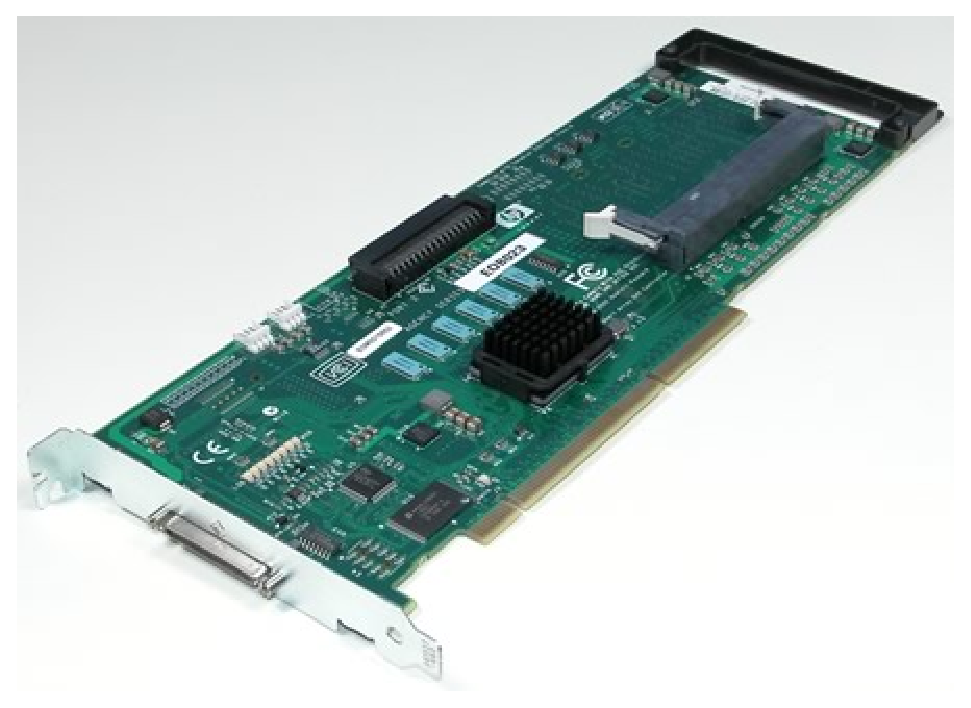
\includegraphics[width=0.65\textwidth]{HP_Smart_Array_642}
\end{center}
  \caption{HP Smart Array 642 controller}
  \label{fig:HP_Smart_Array_642}
\end{figure}


\section{Load balancing strategies}
This section presents a description of the methods for solving the problem presented above in the chapter \ref{chap3:title}. The solutions that we offer are simple, but effectively show the results in practice. We applied them for testing the erasure time of several disks. We remember that the main problem of the research is to minimize the functional of time $T$ or prove that it is not possible because of some limiting factor.

During testing the erasure time of disks with HP Smart Array 642 we applied three load balancing strategies. First two are sequential and the third is parallel, which is working more effectively than the others. Because first two strategies are much slower than the third one, they were tested with the backplane of only 5 disks connected to the internal port of the controller. The third strategy was tested with the enclosure of 14 disks connected to the external port of the controller. In both cases we chose 18.2 GB disks from Compaq. Theoretical expectations about these disks were discussed in the section \ref{sec:theory_est}.

The first strategy performs the complete erasure disk by disk. That means that until the current disk is not erased the program does not start erasure of the next disk. From the section \ref{sec:theory_est} we know that for erasure one 18.2 GB disk we need to send 582 WRITE SAME 10 commands. According to the point that for testing first strategy we took 5 disks we get the following matrix $H_{s1}$ from the model \ref{eq:load_balancing_matrix} for complete erasure:
\begin{equation}
	H_{s1} =
	\begin{pmatrix}
		582 & 0 & 0 & 0 & 0\\
		0 & 582 & 0 & 0 & 0\\
		0 & 0 & 582 & 0 & 0\\
		0 & 0 & 0 & 582 & 0 \\
		0 & 0 & 0 & 0 & 582 \\
	\end{pmatrix}
\end{equation}
From the matrix $H_{s1}$ we can conclude that first strategy has only 5 steps in the algorithm.


Second strategy sends one command per disk and then changes the disk. That means that in this case
matrix $H$ is completely different:
\begin{equation}
\setcounter{MaxMatrixCols}{13}
	H_{s2} =
	\begin{pmatrix}
		1 & 0 & 0 & 0 & 0 &&  		1 & 0 & 0 & 0 & 0 \\
		0 & 1 & 0 & 0 & 0 &&  		0 & 1 & 0 & 0 & 0 \\
		0 & 0 & 1 & 0 & 0 &\ldots&   0 & 0 & 1 & 0 & 0 \\
		0 & 0 & 0 & 1 & 0 &&  		0 & 0 & 0 & 1 & 0 \\
		0 & 0 & 0 & 0 & 1 &&  		0 & 0 & 0 & 0 & 1 \\
	\end{pmatrix}.
\end{equation}
For the second strategy the dimension of matrix $H$ is $5\times2910$. Value $2910$ came from multiplication of number of disks and number of commands that we need to send for the erasure. From the logic of sending commands the devices should be changed quite often, which can be a disadvantage of this strategy. 


The third strategy is using parallel computing, which makes the process for complete erasure much faster. The application creates separate thread for each disk and start sending WRITE SAME commands to that disk. It is obvious that during increasing the amount of disks the value of functional of time will increase too, but slowly, because threads are working completely separately. But important limitations are the speeds of the disk and the bus. As we can see from Figure \ref{fig:conn_model} separate buses $c$ give the possibility to send data from the controller $b$ to the disks $d$. In our situation, only one bus $c$ exists, which is connected to the enclosure containing several disks. If we write information in parallel to several disks the bus speed can be the limitation for data transfer. The maximum speed of the current bus is 320 MB/s. In this case it id difficult to present matrix $H$, because we do not know in which order WRITE SAME commands come to the disks.


\section{Planning dynamic load balancing system}

During whole research we try to find the optimal parameters for sending write commands to the disks, but it seems that we could not say anything before some testing. As it was mentioned in the beginning of the paper load balancing system should take care of these things. Lets discuss what kind of static and dynamic load balancing systems we could provide for our situation. There are so many parameters which depend on the speed of erasure that it is much better to use dynamic load balancing system. But it is also possible to apply static load balancing system using some special conditions.

Main condition that should be fulfilled is knowledge about the cache of the controller. If we know this parameter before the erasure process it is possible to calculate the optimal buffer and optimal number of disks for erasure. The problem is that getting cache from the controller is very specific task and sometimes maybe even impossible one. But using Linux driver we can manually find the maximum value for the transfer buffer. In our situation this value is defined as $MAX\_KMALLOC\_SIZE (4096*512)$, which means that the maximum buffer can not be larger than 2 MB. We do not know exactly if it is cache, but the value looks quite similar to the cache size. If we consider this value as cache we easily can calculate what is the optimal value for the transfer length using 14 disks:
\begin{equation}
	\frac{MAX\_BUFFER}{SECTOR\_SIZE*14} = \frac{4096*512}{512*14} = 292.57.
\end{equation}
In our case we send the buffer with the value of power of 2, that is why 256 is the optimal value, as we can see it also from the result graphic \ref{fig:diff_length_14disks}. And Blancco software sends the buffer exactly with the transfer length 256, but it is optimal when the number of disks is more than 8. Lets calculate the transfer length in case that we have 8 disks:
\begin{equation}
	\frac{MAX\_BUFFER}{SECTOR\_SIZE*14} = \frac{4096*512}{512*8} = 512.
\end{equation}
This fact explains that we should use another transfer length to get an optimal way of sending commands. Moreover, we understand that for 4 disks we need 1024 and for 2 disks - 2048, but it is only theory. In practise, sometimes the results of testing show that some other parameters influence on speed too.




